% -*- TeX-master: "main"; fill-column: 72 -*-

\section{Illustrative examples of the \FBC syntax}
\label{examples}

This section contains a worked example showing the encoding of a model suitable for Flux Balance Analysis using the \FBCPackage.

\subsection{Example one: the basic \FBC syntax}
\label{examples1}
\subsubsection{Kinetic model description}
\begin{figure}[h]
  \centering
  % Requires \usepackage{graphicx}
  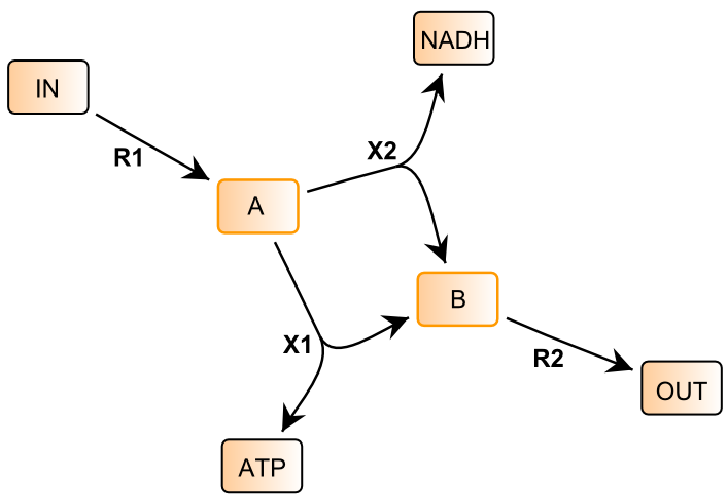
\includegraphics[width=8cm]{examples/spec-example1.pdf}\\
  \caption{\FBC syntax example: a simple four reaction pathway. The
  reactions are \textit{R1}, \textit{R2}, \textit{X1}, \textit{X2} with
  fixed species \textit{IN}, \textit{OUT}, \textit{ATP}, \textit{NADH} and
  variable species \textit{A}, \textit{B}.}
  \label{fig:example1}
\end{figure}

As shown in \ref{fig:example1} this example is a simple four reaction
pathway that transforms metabolite \textit{IN} to \textit{OUT}. The
model was created and analyzed using the \textsf{SBW Flux Balance} \FBC
implementation and CBMPy \citep{sbwfba, cbmpy}. In \SBML each reaction is represented as a chemical process transforming reactants to products, e.g. reaction
\textit{R1} is encoded in XML as (see also the complete example provided
at the end of this section):


%
\exampleFile{examples/spec-example1-reaction.txt}
%
Using the reagent identity and stoichiometry it is possible to compactly
describe this network in terms of its reaction stoichiometry as shown in
\ref{tble:ex1nmat} where each reaction is represented as a column. \newtxt{Each row in the stoichiometric matrix represents the differential equation describing the change of a variable \Species. In \SBML such variable \Species have the attribute \token{boundaryCondition} set to \val{false}. This is in contrast to ``fixed species'' (where the attribute \token{boundaryCondition} is set to \val{true}) which do not appear in the stoichiometric matrix. Please see the \sbmlthreecore specification for more details.}

\begin{table}[h]
  \centering
    \begin{tabular}{c|cccc}
          & R1 & R2 & X1 & X2 \\ \hline
        A & 1 &  0 & -1 & -1 \\
        B & 0 & -1 &  1 &  1 \\
    \end{tabular}
  \caption{Example one: stoichiometric matrix, \Nmat}
  \label{tble:ex1nmat}
\end{table}
%
While the stoichiometry contains the structural properties of the
reaction network the full description of a biological model can, for example, be described as a set of ordinary differential equations (ODE's). Of course other formalisms do exist, but here we will concentrate exclusively on kinetic models where the change in concentration of each variable component in the system ($\frac{ds}{dt}$) is a non-linear function of the rates of the reactions which either create or consume it (the product of the stoichiometric matrix, \Nmat\ and the vector of reaction rates, \vvec).

%
\begin{equation}\label{eqn:kinmod}
  \frac{ds}{dt} = \textbf{Nv}
\end{equation}
%
The formulation of the kinetic model, as shown in
Equation~\ref{eqn:kinmod} is typical of the kind that can already be
described using \sbmlthreecore where the vector \vvec\ would contain
rate equations as a function of parameters and variable species. In a
steady-state, constraint-based model these rates are considered unknowns
and the system of equations can be rewritten as a set of linear
constraints (see Equation~\ref{eqn:kinmodsteady}):


%
\begin{equation}\label{eqn:kinmodsteady}
  \textbf{NJ} = 0
\end{equation}
%
Note that the rate vector \vvec\ is now represented as the steady-state
flux vector \Jvec. However, in order to perform a typical steady-state
analysis such as flux balance analysis (FBA) we need to include more
information into the model description. \sbmlthreecore does not have an
unambiguous way of encoding either a capacity constraint or an objective function and for this we need to use the additional constructs provided by the \FBCPackage. In the following sections the same model data is shown
encoded as XML and as a linear program (LP) in the commonly used IBM\textsuperscript{\tiny{TM}} \textsf{CPLEX} format.


\subsubsection{Flux Bounds}
\label{examples1:fluxbound}
\newtxt{A capacity constraint or flux bound describes the limits that the flux through a certain reaction may attain at steady state}. In this example the maximum limit (upper bound) on the flux through reaction \textit{R1} is set to be one with the minimum value (lower bound) set to zero (with an arbitrary unit of flux). In LP format this may be written as:
%
\exampleFile{examples/spec-example1-bnd.lp}
%
the same information encoded as XML:
%
\exampleFile{examples/v2harmony-spec-example1-bnd.txt}

\medskip
\subsubsection{Objective function}
\label{examples1:objfunc}
This described a target which can be maximized or minimized: in this
example the flux through reaction \textit{R2} will be
\textit{maximized}.

%
\exampleFile{examples/spec-example1-obj.lp}
%
the same information encoded as XML:
%
\exampleFile{examples/spec-example1-obj.txt}

\subsubsection{Complete worked example}
\label{examples1:complete}
To conclude we show how the complete model described in
\ref{fig:example1} encoded as both an LP and as XML. Formulated as an LP
the problem can be written as:

%
\exampleFile{examples/spec-example1.lp}
%
Solving this we find that maximization of flux through \textit{R2}
gives an optimal solution $R2 = 1$, shown in Equation~\ref{egn:ex1sol1}, with one possible solution
for \Jvec.
\begin{equation}\label{egn:ex1sol1}
  \left(
    \begin{array}{cccc}
        1 &  0 & -1 & -1 \\
        0 & -1 &  1 &  1 \\
    \end{array}
  \right)
  \left(
    \begin{array}{c}
        1.0 \\
        \textbf{1.0} \\
        0.0 \\
        1.0 \\
    \end{array}
  \right)
  = \textbf{0}
\end{equation}

Finally we provide the complete model, described above, encoded using the \FBCPackage:
%
\exampleFile{examples/v2harmony-spec-example1.txt}
